\documentclass[11pt]{article}

\usepackage{graphicx} % for including graphics
\usepackage{amsmath} % useful maths macros, including \text
\usepackage{listings}
\usepackage{gensymb}
\usepackage{textcomp}
\usepackage{afterpage}
\usepackage{apacite}

\usepackage{caption}
\usepackage{subcaption}

\usepackage[style=ieee]{biblatex}
\addbibresource{shared_resources/master.bib}

% \usepackage{multicol}
% \usepackage{float}
\usepackage[a4paper, total={6.5in, 7.5in}]{geometry} % set the paper/text sizes
\def\apj{Astrophysical Journal}
\def\prd{Physical Review D}
\def\apjl{Astrophysical Journal Letters}



\title{\bf{Status and overview of deep-learning enhancements to gravitational wave parameter estimation}\\~\\
\large Submission of technical literature review}



\author{2259886}

\begin{document}
\maketitle

% section planning:

\section*{Introductory gravitational waves (detail: pipeline and detections, progress, sensitivity, ASD}

From their first hypothesis~\cite{einstein1} to the first direct detection of signal from binary black hole coalescence~\cite{abbott2016observation} by Advanced LIGO~\cite{advancedLIGO} and Advanced VIRGO~\cite{advacnedVIRGO} square-kilometre interferometers, we find ourselves in an exciting new epoch of gravitational physics. With the first two observing runs~\cite{BBHO1,gwtc1} and the first half of the third run~\cite{gwtc2} findings published along with corresponding public data release, the interest in gravitational waves is at an all time high (see figure~\ref{fig:wos}). Improvements in detector sensitivity between runs (see figure~\ref{fig:asd}) has allowed a much increased candidate detection-rate, of which more are to be published from the O3b run (note was cut short by COVID-19) to *insert approx dection rate for O3a* (see figure~\ref{fig:events}).

\begin{figure}[t!]
    \centering
    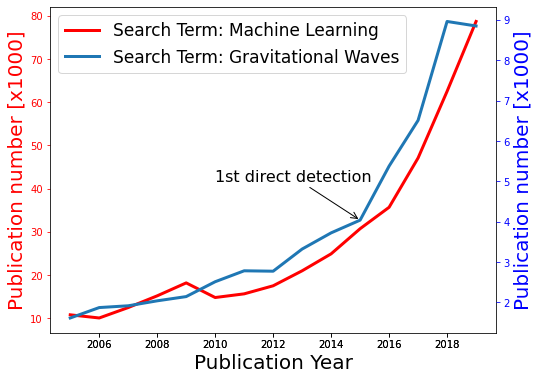
\includegraphics[width=.6\linewidth]{shared_resources/shared_figs/wos.png}
    \caption{Caption}
    \label{fig:wos}
\end{figure}

\subsection*{What are grav waves and how to detect - focus on transients (not spec BBH yet)}

\begin{figure}[htb]
    \centering
    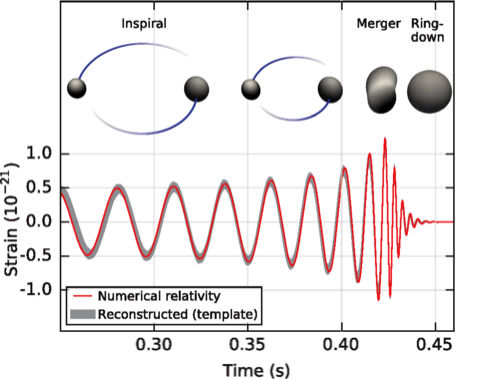
\includegraphics[width=.6\linewidth]{shared_resources/shared_figs/inspiral.png}
    \caption{Caption}
    \label{fig:events}
\end{figure}

\subsection*{More info on detection pipelines - intro problems/ improvements for Bayesian and ML}


\section*{Bayesian Intro (usefulness in pipeline)}


\section*{Introductory machines learning}

\section*{Plan for final report intro}

I have kept this literature review very general as, by virtue of such a complex topic that is new to me, and the cutting-edge nature of the research the exact nature of my project direction is being modified weekly. Also, by nature of the very specific methods of PE,sampling, CVAE etc, I have found that I have not grasped all aspects quite yet, so cannot write about them. The main things I am looking to work on before a final draft of intro will be completed:
\begin{itemize}
  \item Variational inference (VI) methods (expecting a presentation within the IGR-data group week beginning , specifically Conditional Variational Autoencoders (CVAE)
  \item Publication of O3b catalog
  \item Better practical working knowledge of tensorflow~\cite{tensorflow}
\end{itemize}


\begin{figure}[htb]
     \centering
     \begin{subfigure}[t]{0.47\linewidth}
         \centering
         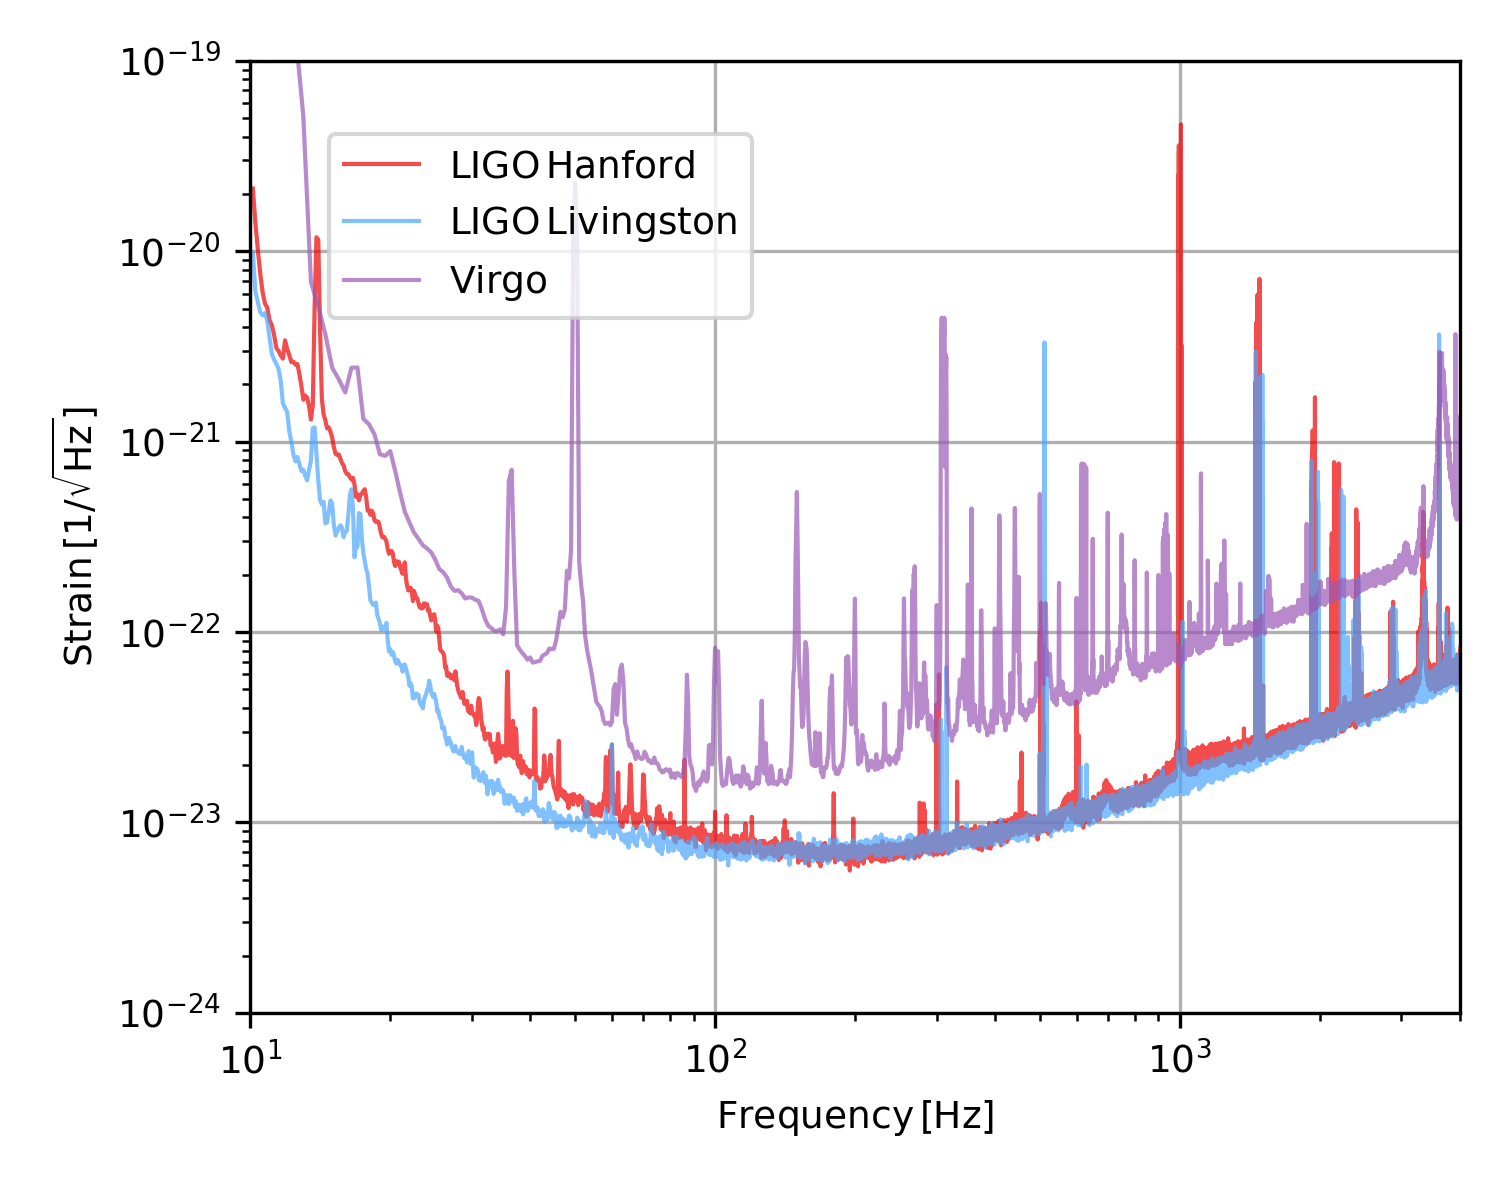
\includegraphics[width=\linewidth]{shared_resources/shared_figs/o2_asd.png}
     \end{subfigure}
     \begin{subfigure}[t]{0.47\linewidth}
         \centering
         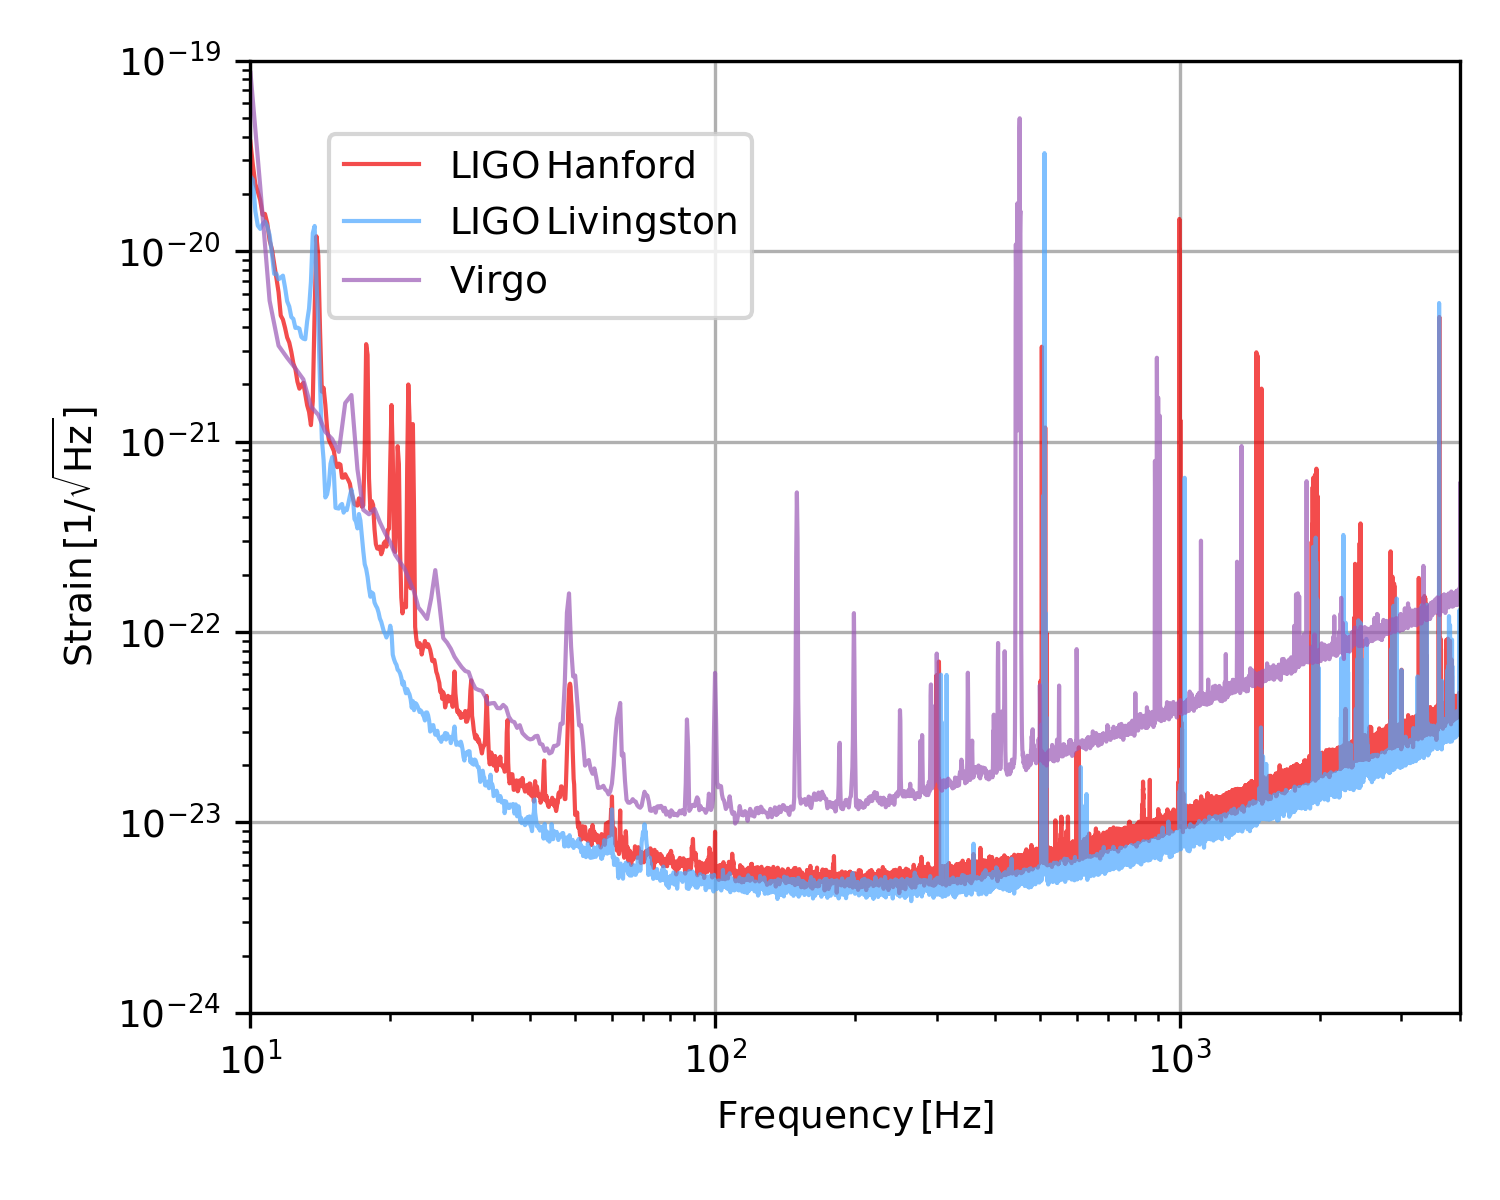
\includegraphics[width=\linewidth]{shared_resources/shared_figs/o3a_asd.png}
     \end{subfigure}
     \vspace*{-7mm}
     \caption{Full caption}
     \label{fig:asd}
\end{figure}

\begin{figure}[htb]
    \centering
    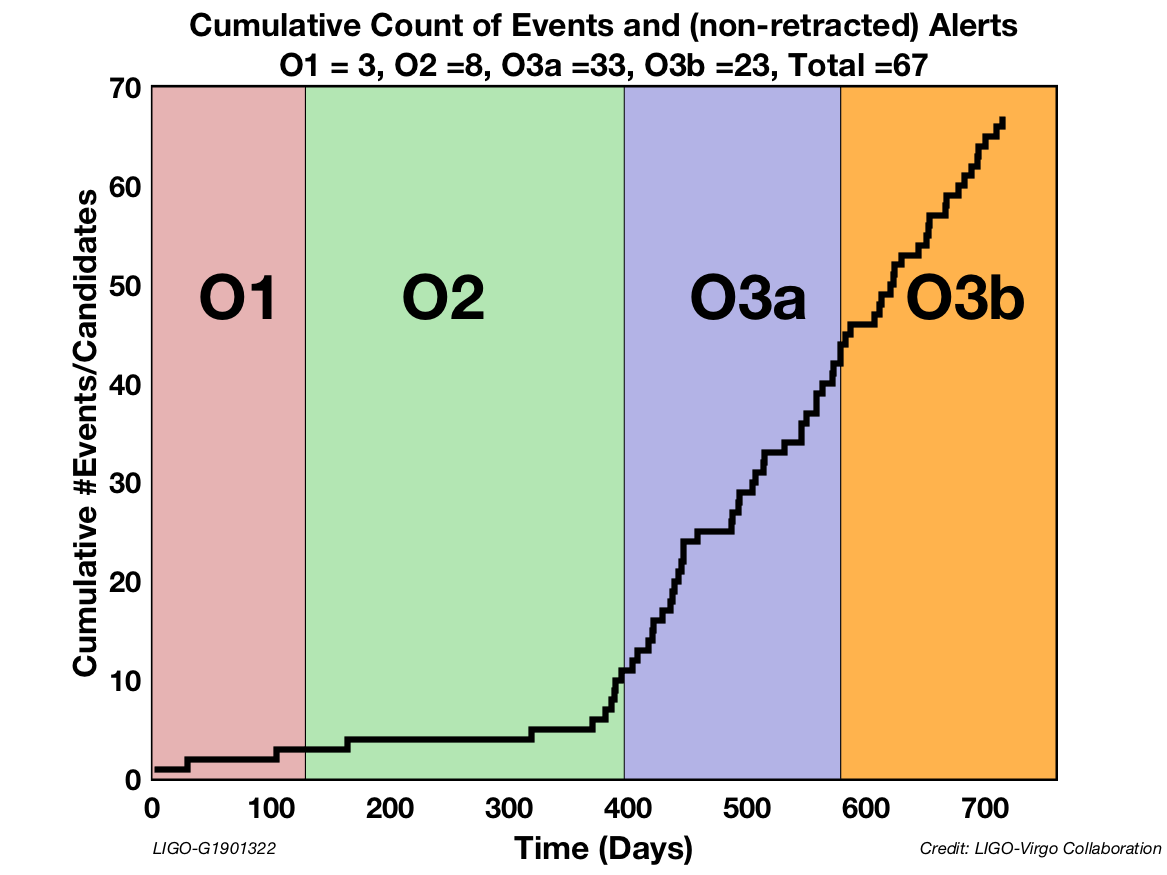
\includegraphics[width=.75\linewidth]{shared_resources/shared_figs/number_events.png}
    \caption{Caption}
    \label{fig:events}
\end{figure}





\newpage

\printbibliography



























































































\end{document}
